%!TEX ROOT=formularioMatematica.tex

\section{Derivate}\label{sec:derivate}

Il concetto di derivata è uno dei concetti fondamentali della matematica. È la base delle equazioni
differenziali, integrali, calcolo infinitesimale e molto altro.\\
Per arrivare ad una definizione di derivata, si possono prendere due strade, le stesse che Newton e 
Leibniz intrapresero. Osserveremo il metodo di Leibniz in quanto è più matematico. Quello di Newton
invece ha più riferimenti con la fisica.\\
Leibniz si era posto il problema di come trovare la tangente in un punto di una curva. Ad esempio
\begin{center}
  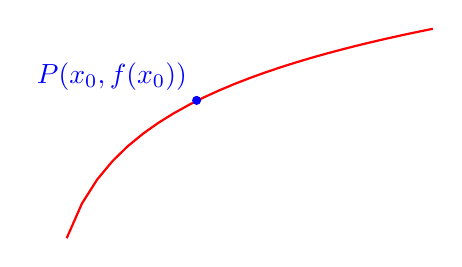
\begin{tikzpicture}
    \tkzInit[xmin=0,ymin=-1,xmax=5,ymax=3]
    \tkzGrid
    \tkzAxeXY
    \draw[domain=0.35:5, thick, red] plot({\x}, {ln(\x)});
    \filldraw[blue] (2,0.7) circle (0.05)
      node[above left]{$P(x_0,f(x_0))$};
  \end{tikzpicture}
\end{center}
come troviamo la tangente ad $f(x)$ (in rosso) in $P$ (in blu)? L'idea qui è quella di fissare un
altro punto ($Q$) di coordinate ($(x,f(x))$) e trovare la retta che passa tra questi due punti che,
ovviamente, risulterà secante alla curva. Poi si avvicinerà sempre di più il punto $Q$ a $P$ in modo
che la retta tra i due punti, risulti in definitiva tangente alla curva.
\begin{center}
  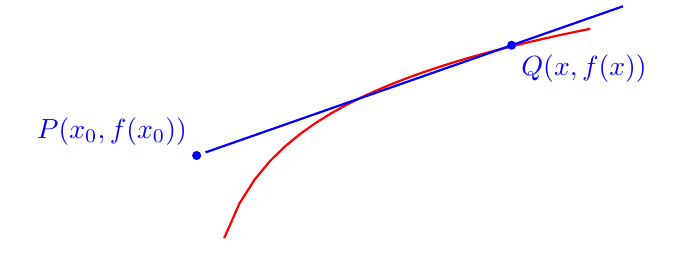
\begin{tikzpicture}
    \coordinate (P) at (2,0.70);
    \coordinate (Q) at (4,1.4);
    \tkzInit[xmin=0,ymin=-1,xmax=5,ymax=3]
    \tkzGrid
    \tkzAxeXY

    \draw[domain=0.35:5, thick, red] plot({\x}, {ln(\x)});
    \draw[blue, thick, shorten >= -1.5cm, shorten <= -2cm] (P) -- (Q);

    \filldraw[blue] (Q) circle (0.05)
      node[below right]{$Q(x,f(x))$};
    \filldraw[blue] (0,0) circle (0.05)
      node[above left]{$P(x_0,f(x_0))$};
  \end{tikzpicture}
\end{center}
Ora noi vorremmo trovare questa retta. Per prima cosa, troviamo il coefficiente angolare
\begin{equation*}
  m_{PQ} = \frac{y_Q-y_P}{x_Q-x_P} = \frac{f(x)-f(x_0)}{x-x_0}
\end{equation*}
Questa frazione, è definita \textbf{rapporto incrementale nel punto $x_0$}. Spesso è scritta anche
come 
\begin{equation*}
  m = \frac{\Delta f}{\Delta x}
\end{equation*}
o, ponendo $x-x_0 = h$
\begin{equation*}
  m = \frac{f(x_0+h)-f(x_0)}{h}
\end{equation*}
Ora per trovare quello della tangente, dobbiamo avvicinare $Q$ a $P$, quindi
\begin{equation*}
  m_t = \lim\limits_{x\to x_0} \frac{f(x)-f(x_0)}{x-x_0} = 
  \lim\limits_{h\to0} \frac{f(x_0+h)-f(x_0)}{h}
\end{equation*}
Se questo limite esiste ed è finito, la funzione $f$ si dice \emph{derivabile} in $x_0$ e si pone
\begin{equation*}
  f'(x_0) = \lim\limits_{x\to x_0} \frac{f(x)-f(x_0)}{x-x_0} = 
  \lim\limits_{h\to0} \frac{f(x_0+h)-f(x_0)}{h}
\end{equation*}
Altre notazioni sono
\begin{equation*}
  \Dif f(x_0)\quad\text{e}\quad \frac{\dif f}{\dif x}(x_0)
\end{equation*}

\subsection{Teoremi sulle derivate}
Tra i teoremi sulle derivate e le derivate delle funzioni elementari, si potranno calcolare con
estrema facilità tutte le derivate che si proporranno.

\subsubsection{Somma}
\begin{equation*}
  \Dif \left[ f(x)\pm g(x) \right] = \Dif f(x)\pm\Dif g(x)
\end{equation*}
Si estenda la proprietà al numero di funzioni desiderato. Si faccia comunque la somma algebrica.

\subsubsection{Prodotto}
\begin{equation*}
  \Dif \left[ f(x)\cdot g(x) \right] \left[ \Dif f(x) \right]g(x) + f(x)\left[ \Dif g(x) \right]
\end{equation*}
Si noti che se $g(x) = k\lor f(x) = k$,
\begin{equation*}
  \Dif \left[ k\cdot f(x) \right] = k\Dif f(x)
\end{equation*}
Si noti che per un numero $\alpha\in\mathbb{R}$ di funzioni $f(x)$, il loro prodotto diventerebbe
una potenza, in particolar modo
\begin{equation*}
  \Dif[f(x)]^\alpha = \alpha f'(x)[f(x)]^{\alpha-1}
\end{equation*}

\subsubsection{Quoziente}
\begin{equation*}
  \Dif \left( \frac{f(x)}{g(x)} \right) = \frac{[\Dif f(x)]g(x)-f(x)\Dif g(x)}{[g(x)]^2}
\end{equation*}

\subsubsection{Derivata di una funzione inversa}
\begin{equation*}
  \Dif f^{-1}(x_0) = \frac{1}{\Dif f(x_0)}
\end{equation*}

\subsubsection{Derivata di una funzone composta}
\begin{equation*}
  \Dif [f(g(x))] = \Dif f(g(x))\cdot\Dif g(x)
\end{equation*}
Se sono presenti più funzioni si estenda di conseguenza. Quindi
\begin{equation*}
  \Dif [f(g(h(x)))] = \Dif f(g(h(x)))\cdot\Dif g(h(x))\cdot\Dif h(x)
\end{equation*}
e così via per altre funzioni.

\subsection{Derivate fondamentali}
Verranno ora riportate le derivate fondamentali delle funzioni elementari. Con queste e con i
teoremi sarà possibile trovare una qualunque derivata di una qualunque funzione.
\tablefirsthead{\toprule \textbf{Funzione} & \textbf{Derivata}\\ \midrule}
\tablehead{\textbf{Funzione} & \textbf{Derivata}\\ \midrule}
\tablelasttail{\bottomrule}
\begin{center}
  \begin{xtabular}{M{2cm} M{5cm}}
    $c\,(c\in\mathbb{R})$ & $0$\\ \midrule
    $f(x)^\alpha\, (\alpha\in\mathbb{R})$ & $\alpha x^{\alpha-1}f'(x)$\\ \midrule
    $\sin f(x)$ & $\cos(f(x))f'(x)$\\ \midrule
    $\cos f(x)$ & $-\sin(f(x))f'(x)$\\ \midrule
    $\tan f(x)$ & $(1+\tan^2 f(x))f'(x)=\frac{f'(x)}{\cos^2f(x)}$\\ \midrule
    $\cot f(x)$ & $-(1-\cot^2f(x)f'(x)=-\frac{f'(x)}{\sin^2f(x)}$\\ \midrule
    $\log_a f(x)$ & $\frac{f'(x)}{f(x)}\log_a e$\\ \midrule
    $a^{f(x)}$ & $a^{f(x)}\ln af'(x)$\\ \midrule
    $\arcsin f(x)$ & $\frac{f'(x)}{\sqrt{1-f(x)^2}}$\\ \midrule
    $\arccos f(x)$ & $-\frac{f'(x)}{\sqrt{1-f(x)^2}}$\\ \midrule
    $\arctan f(x)$ & $\frac{f'(x)}{1+f(x)^2}$\\ \midrule
    $\arccot f(x)$ & $-\frac{f'(x)}{1+f(x)^2}$\\
  \end{xtabular}
\end{center}
Si noti che è presente anche questa formula
\begin{equation*}
  \Dif[f(x)]^{g(x)}=[f(x)]^{g(x)} \left[ \Dif g(x)\ln f(x)+g(x) \frac{\Dif f(x)}{f(x)} \right]
\end{equation*}
che risulta essere molto difficile da ricordare ma è facilmente ricavabile sfruttando la nota
caratteristica
\begin{equation*}
  f(x)^{g(x)} = e^{g(x)\ln f(x)}
\end{equation*}

\subsection{Derivate successive}
Le derivate successive sono derivate di derivate di derivate \ldots\\
La notazione può essere o usando numeri romani sopra la funzione
\begin{equation*}
  f^I(x),\,f^{II}(x),\,f^{III}(x)
\end{equation*}
oppure con numeri arabi come pedice
\begin{equation*}
  f_1(x),\,f_2(x),\,f_3(x)
\end{equation*}
o infine usare gli apostrofi conseguentamente (da preferirsi per numeri piccoli)
\begin{equation*}
  f'(x),\,f''(x),\,f'''(x)
\end{equation*}

\subsection{Rapporto tra continuità e derivabilità}
Andiamo a verificare se dalla continuità di una funzione, possiamo dedurre la derivabilità.
Prendiamo come funzione
\begin{equation*}
  f(x) = \abs{x}
\end{equation*}
È continua in quanto $\mathbb{R}$ è il suo dominio e il suo codominio. L'unico punto che può
essere di qualche difficoltà è $x_0=0$. Quindi andiamo a verificare la derivata sinistra 
e la derivata destra.
\begin{equation*}
  f_+'(x) = \lim\limits_{x\to0^+} \frac{\abs{x}}{x} = 1
\end{equation*}
\begin{equation*}
  f_-'(x) = \lim\limits_{x\to0^-} \frac{\abs{x}}{x} = -1 
\end{equation*}
Dato che le due derivate sono diverse,
\begin{equation*}
  \not\exists\,f'(0)
\end{equation*}
Quindi \textbf{se $f(x)$ è continua in $x_0$ non è detto che sia derivabile in quel punto}.\\
[\baselineskip]
Ora invece proviamo a vedere se
\begin{equation*}
  \lim\limits_{x\to x_0}f(x) = f(x_0)
\end{equation*}
Scriviamo l'identità
\begin{equation*}
  f(x) = f(x)
\end{equation*}
Addizioniamo e sottraiamo $f(x_0)$ e dividiamo e moltiplichiamo $x-x_0$, otteniamo
\begin{equation*}
  f(x) = f(x_0)+\frac{f(x)-f(x_0)}{x-x_0}(x-x_0)
\end{equation*}
Quindi ora possiamo scrivere
\begin{equation*}
  \lim\limits_{x\to x_0} f(x)=
  \lim\limits_{x\to x_0}\left[ f(x_0)+\overbrace{\frac{f(x)-f(x_0)}{x-x_0}}^{f'(x_0)}
  \overbrace{(x-x_0)}^{0}\right] = f(x_0)
\end{equation*}
Abbiamo quindi dimostrato che \textbf{se $f(x)$ è derivabile in $x_0$, allora $f(x)$ è continua}. 

\subsection{Punti di non derivabilità}
I punti di non derivabilità sono quei punti che vengono fuori da
\begin{equation*}
  \mathcal{D}_f - \mathcal{D}_{f'} 
\end{equation*}
Esistono 3 tipi di non derivabilità.
\subsubsection{Punti angolosi}
$x_0$ è un punto angoloso per $f(x)$ se $f_+'(x)$ e $f_-'(x) $sono finiti (o al massimo uno è 
infinito) e $f_+'(x)\neq f_-'(x)$.\\
Un chiaro esempio si vede in $f(x)=\abs{x^2-c}$.
\begin{center}
  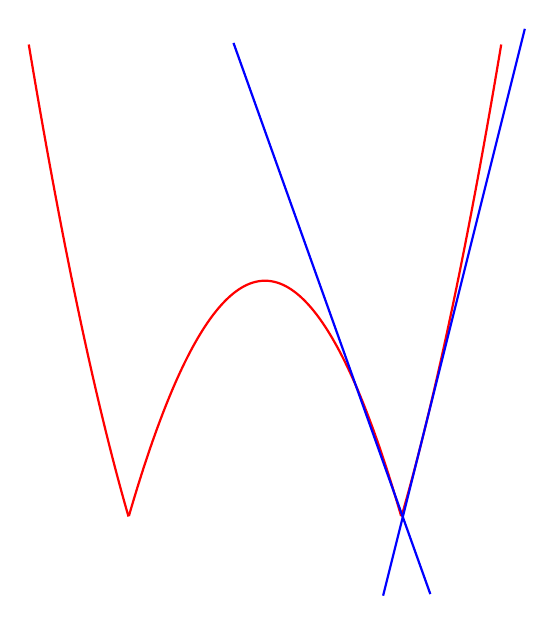
\begin{tikzpicture}
    \tkzInit[xmin=-4,ymin=-1,xmax=4,ymax=6]
    \tkzGrid
    \tkzAxeXY
    \draw[domain=-3:3, red, thick, samples=500] plot(\x,{abs(\x*\x-3)});
    \draw[domain=-0.4:2.1, blue, thick] plot(\x,{-2.8*\x+4.9});
    \draw[domain=1.5:3.3, blue, thick] plot (\x, {4*\x-7});
  \end{tikzpicture}
\end{center}
I punti in cui $f(x)=0$ sono detti angolosi in quanto le due tangenti verso destra e verso sinistra
sono diverse.

\subsubsection{Cuspidi}
$x_0$ si definisce cuspide se
\begin{equation*}
  \lim\limits_{\Delta x\to 0^-} \frac{\Delta f}{\Delta x}=-\infty\quad
  \lim\limits_{\Delta x\to 0^+} \frac{\Delta f}{\Delta x}=+\infty
\end{equation*}
I due tipici cuspidi sono
\begin{center}
  \begin{tikzpicture}
    \clip (-3.5,-1.5) rectangle (6,4);
    \tkzInit[xmin=-3,ymin=-1,xmax=3,ymax=3]
    \tkzGrid
    \tkzAxeXY
    \draw[red, thick] (-3,2) to[out=0,in=90] (0,0);
    \draw[red, thick] (3,2) to[out=180,in=90] (0,0);
  \end{tikzpicture}
\end{center}
e
\begin{center}
  \begin{tikzpicture}
    \clip (-3.5,-1.5) rectangle (6,4);
    \tkzInit[xmin=-3,ymin=-1,xmax=3,ymax=3]
    \tkzGrid
    \tkzAxeXY
    \draw[red, thick] (-3,0) to[out=0,in=270] (0,2);
    \draw[red, thick] (3,0) to[out=180,in=270] (0,2);
  \end{tikzpicture}
\end{center}

\subsubsection{Flessi a tangente verticale}
$x_0$ è un flesso se
\begin{equation*}
  \lim\limits_{\Delta x\to0} \frac{\Delta f}{\Delta x} = \pm\infty
\end{equation*}
I due tipici flessi sono
\begin{center}
  \begin{tikzpicture}
    \clip (-3.5,-1.5) rectangle (6,4);
    \tkzInit[xmin=-3,ymin=-1,xmax=3,ymax=3]
    \tkzGrid
    \tkzAxeXY
    \draw[red, thick] (-3,-1) to[out=0,in=270] (0,1);
    \draw[red, thick] (3,3) to[out=180,in=90] (0,1);
  \end{tikzpicture}
\end{center}
e
\begin{center}
  \begin{tikzpicture}
    \clip (-3.5,-1.5) rectangle (6,4);
    \tkzInit[xmin=-3,ymin=-1,xmax=3,ymax=3]
    \tkzGrid
    \tkzAxeXY
    \draw[red, thick] (-3,3) to[out=0,in=90] (0,1);
    \draw[red, thick] (3,-1) to[out=180,in=270] (0,1);
  \end{tikzpicture}
\end{center}

\subsection{Problemi di ottimizzazione}
I problemi di ottimizzazione sono problemi come ad esempio trovare l'area massima di un rettangolo
sotto una curva, il volume minimo di un solido che soddisfi certe condizioni, \ldots. I passi per
risolvere questi esercizi sono i seguenti
\begin{enumerate}
  \item Scegliere una $x$ appropriata
  \item Trovare una funzione da ottimizzare
  \item Determinare un intervallo $I(x)$
  \item Fare la derivata della funzione per ricavarne massimi e minimi
\end{enumerate}
Prendiamo per esempio il seguente problema: data la funzione $f(x)=\sqrt{x}$, si trovi il punto 
$P\in f(x)$ più vicino a $(4,0)$.\\
Come procedere? Innanzitutto bisogna identificare il punto $P$. Esso, dato che appartiene alla 
funzione, ha coordinate $P(x,\sqrt{x})$. La distanza è data dalla relazione pitagorica
\begin{equation*}
  d = \sqrt{(x-4)^2+(\sqrt{x})^2} = \sqrt{x^2+16-8x+x}= \sqrt{x^2-7x+16} 
\end{equation*}
A questo punto, dobbiamo minimizzare questa funzione. Prendiamone la derivata
\begin{equation*}
  d' = \frac{2x-7}{2\sqrt{x^2-7x+16}}
\end{equation*}
Ora non resta che determinare il segno della derivata
\begin{center}
  \begin{tikzpicture}
    \drawSign{2*\x-7}{2}{5}{0.25}{}
  \end{tikzpicture}
\end{center}
Questo significa che per $x=\frac{7}{2}$ abbiamo un punto di minimo relativo! Ovvero il punto della
funzione che è più vicino a $(4,0)$. Quindi si ha che
\begin{equation*}
  P \left( \frac{7}{2}, \sqrt{\frac{7}{2}}  \right)
\end{equation*}
